\documentclass[a4paper,11pt,titlepage]{article}
\usepackage{graphicx,
	float,
	hyperref}

\DeclareGraphicsExtensions{.png,.eps}
\renewcommand{\arraystretch}{1.3}

\widowpenalty=3000
\clubpenalty=3000

\pagestyle{fancy}
\author{Sam Smith}
\title{OrbSim User Manual}
\date{}
\begin{document}
\maketitle
\tableofcontents
\clearpage

\section{Introduction}
Orbsim is a program designed to simulate the orbits of the planets and to help
the user to understand Kepler's laws of planetary motion. It is available as
compiled executables for Windows and Linux, and as the source files. This user
manual will help a user to understand how to install and use the program. \\

Orbsim allows the user to add bodies to the system, remove bodies from the
system, save the system to a file and load the system from a file. This user
manual describes, in detail how to perform any of these actions and any errors
that may occur when doing this.

\section{Installation}
OrbSim is distributed as an executable file. To use it, download the zip file
from one of the links below. 

\begin{description}
	\item[Windows:] \url{https://db.tt/p0j3k02u}
	\item[Linux:] \url{https://db.tt/90ipAFdh}
\end{description}

When the dialog box appears select open file, wait for it to download and
extract it to a location of your choice. The zip should contain two files, and
executable and a file called bodies.txt. These should be extracted to the same
location. Once they have been extracted, navigate to the files and run the
executable.

\section{Using OrbSim}

After starting the program, you should see this (the actual appearance may vary
from system to system).
\begin{figure}[H]
	\centering
	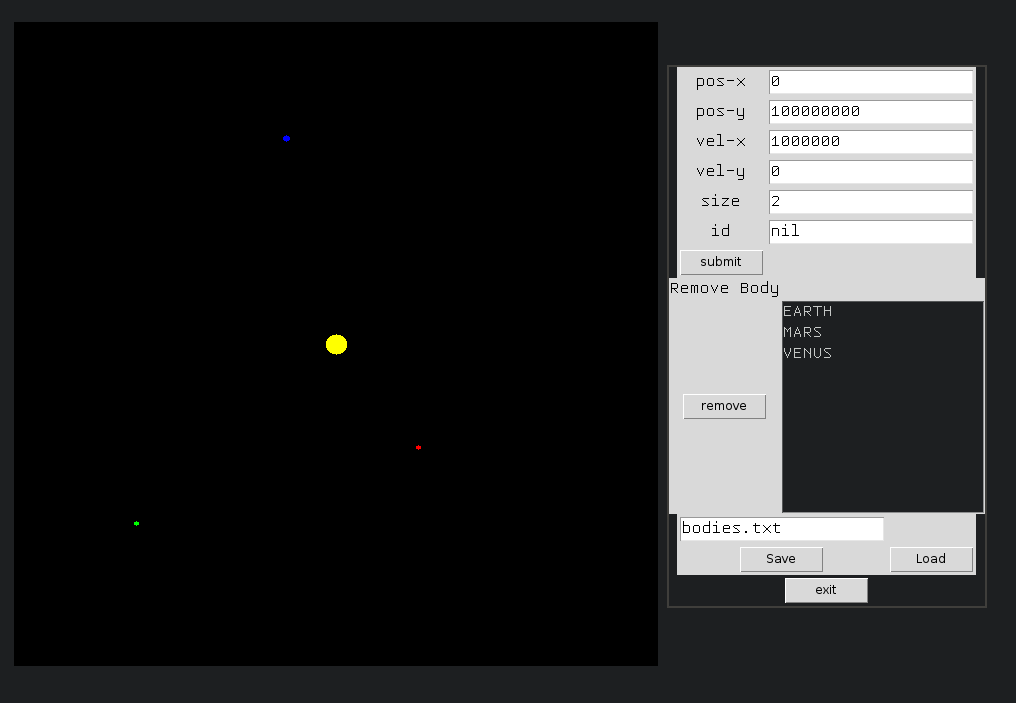
\includegraphics[width=0.8\textwidth]{../img/start.png}
	\caption{What the program might look like on a Linux system}
\end{figure}

Or something like this:

\begin{figure}[H]
	\centering
	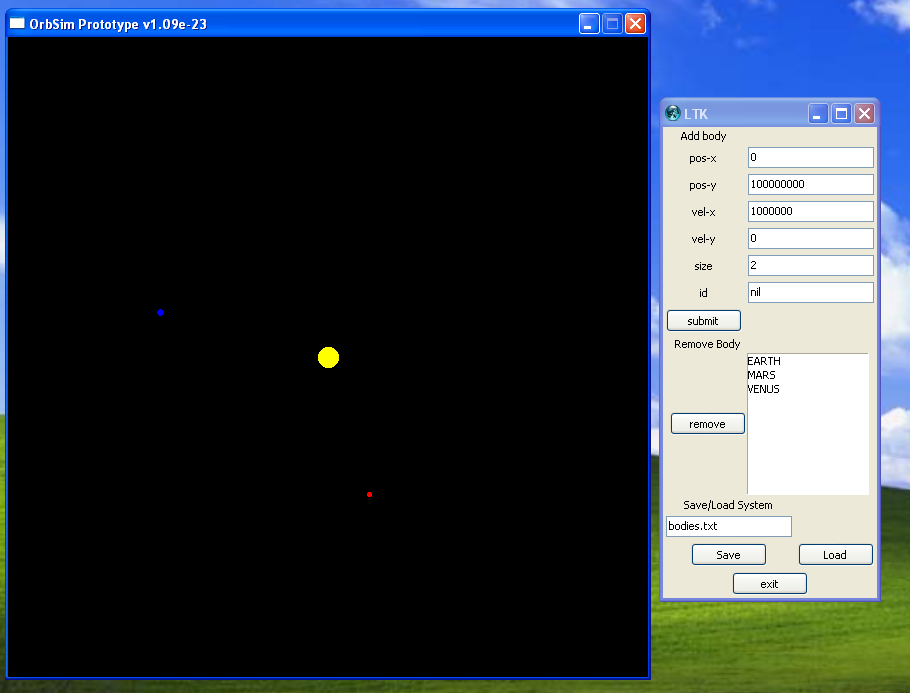
\includegraphics[width=0.8\textwidth]{../img/win.png}
	\caption{What the program might look like on a Windows system}
\end{figure}
The simulation should be running already, if it isn't try closing the program
and opening it again.

\subsection{Adding a body to the simulation}
To add a body to the simulation, just click the submit button in the menu. A new
body should appear in the system and start  orbiting the sun. The supplied
values are good values for a simple elliptical orbit. The parameters in the add
body section of the menu can be used to change where the body starts, how fast
it goes and how it looks. A higher pos-x value will make the body start further
to the right. A higher pos-y value will make the body start further above the
sun. A higher vel-x value will make the body start moving faster towards the
right of the screen, and a higher vel-y value will make the body start moving
faster towards the top of the screen. The size value is the radius of the body
in pixels and the id is the bodies identifier, which is used in the list in the
remove body section.
\begin{figure}[H]
	\centering
	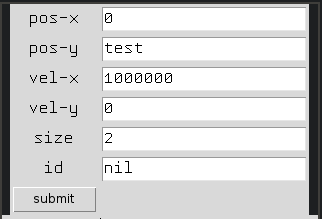
\includegraphics[width=0.5\textwidth]{../img/addman.png}
	\caption{The part of the menu used for adding a body}
\end{figure}

\subsection{Removing a body from the simulation}
To remove a body from the system, select the body to remove and click the remove
button. If no body is selected an error message will appear to ask you to select
a body.
\begin{figure}[H]
	\centering
	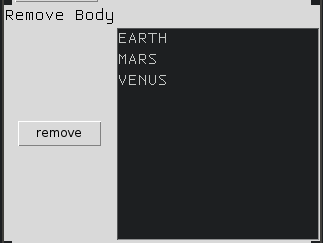
\includegraphics[width=0.5\textwidth]{../img/remove.png}
	\caption{The part of the menu used for removing a body}
\end{figure}

\subsection{Saving the current simulation state}
To save the system, click the save button near the bottom of the menu. It is
advised that you change the filename first because bodies.txt is loaded by
default, and stores the default system.

\subsection{Loading a saved simulation state}
To load a system, enter the name of the file you wish to load and click load.
\begin{figure}[H]
	\centering
	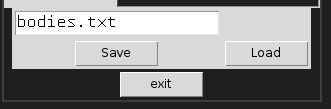
\includegraphics[width=0.6\textwidth]{../img/saveload.png}
	\caption{The part of the menu used for saving and loading the system}
\end{figure}

\section{Common Errors}
\subsection{Invalid integer when adding bodies}
When adding a body to the simulation, this error may occur.
\begin{figure}[H]
	\centering
	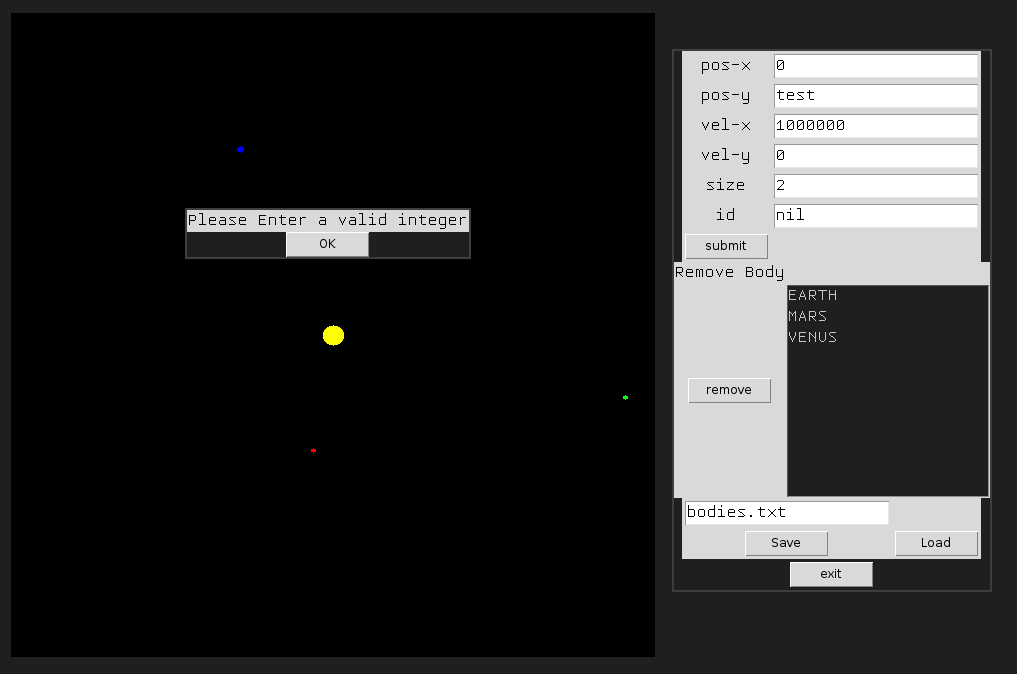
\includegraphics[width=0.8\textwidth]{../img/add2.png}
\end{figure}
To prevent it, make sure that the position and velocity values are all between
10000 and 10000000000, and the size is below 100. If it continues to happen try
closing the program and opening it again.

\subsection{No body selected to remove}
When trying to remove a body, this error message may appear.
\begin{figure}[H]
	\centering
	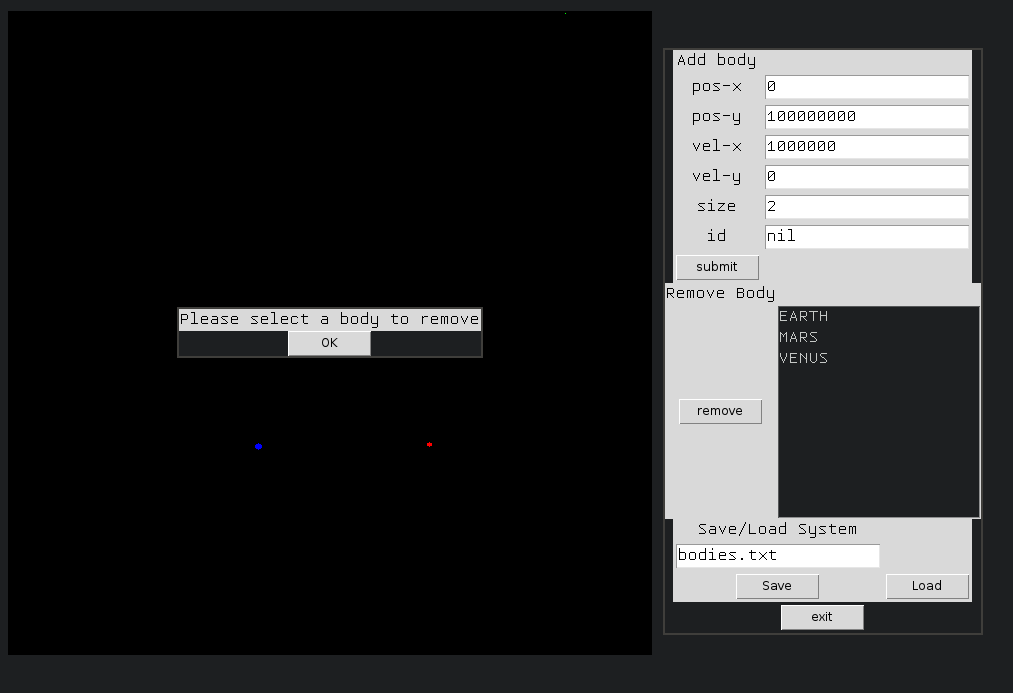
\includegraphics[width=0.8\textwidth]{../img/rm3.png}
\end{figure}

If it does, click OK and try selecting the body you would like to remove again.
If it continues to happen try adding a new body and removing it, if it still
continues try closing the program and opening it.

\subsection{Invalid file name while saving}
Some characters aren't allowed in file names. If you get this error your file
name contains one or more of these characters. The characters that aren't
allowed depends on the operating system that you are using. Currently only
Windows and Linux are supported. The characters that aren't allowed are: \\

\begin{tabular}{l|l}
	Windows & \textless, \textgreater, :, /, \textbackslash{}, \textbar, ?,
	* \\ \hline
	Linux & /, ;, :, \textbar
\end{tabular}
\begin{figure}[H]
	\centering
	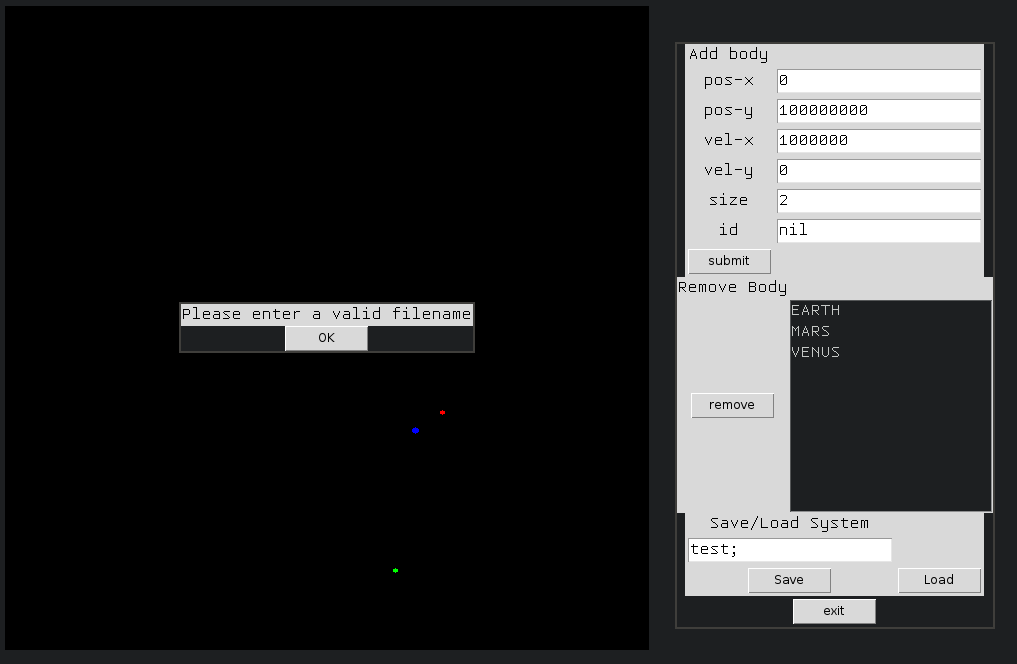
\includegraphics[width=0.8\textwidth]{../img/save.png}
\end{figure}

\subsection{File does not exist}
While attempting to load a saved system this error may appear. This means that
the file you are trying to load does not exist. If this happens check the folder
where the OrbSim executable is stored and make sure that the file you are trying
to load exists. If it does and the error persists, try closing the program and
opening it again. If it continues the file you are trying to load probably
contains errors and cannot be loaded.
\begin{figure}[H]
	\centering
	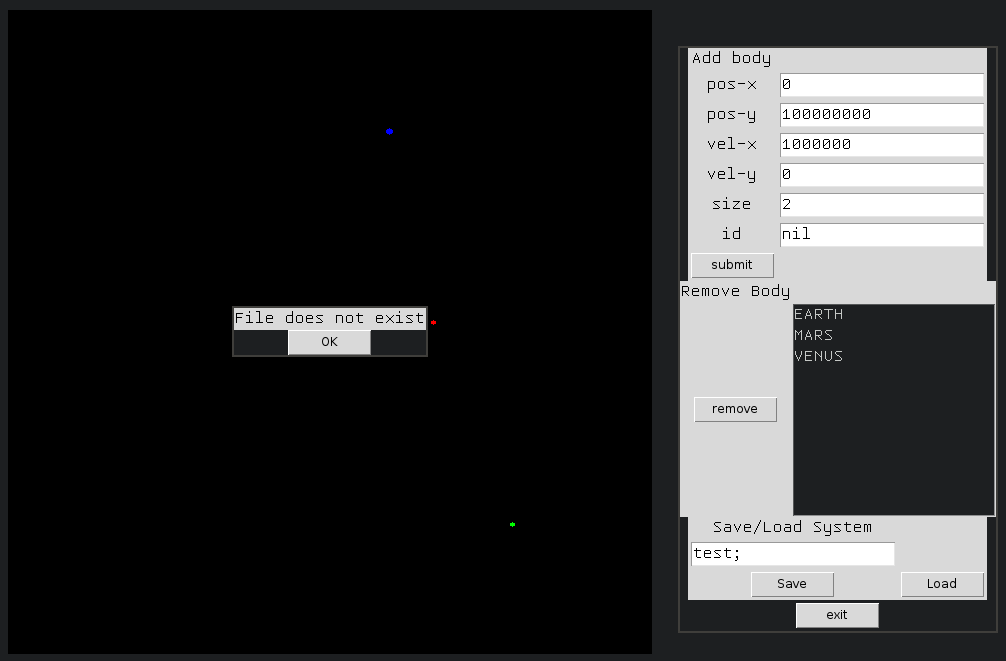
\includegraphics[width=0.8\textwidth]{../img/load.png}
\end{figure}

\end{document}
